\documentclass{beamer}

\pdfmapfile{+sansmathaccent.map}


\mode<presentation>
{
  \usetheme{Warsaw} % or try Darmstadt, Madrid, Warsaw, Rochester, CambridgeUS, ...
  \usecolortheme{crane} % or try seahorse, beaver, crane, wolverine, ...
  \usefonttheme{serif}  % or try serif, structurebold, ...
  \setbeamertemplate{navigation symbols}{}
  \setbeamertemplate{caption}[numbered]
} 


%%%%%%%%%%%%%%%%%%%%%%%%%%%%
% itemize settings

\definecolor{myhotpink}{RGB}{255, 80, 200}
\definecolor{mywarmpink}{RGB}{255, 60, 160}
\definecolor{mylightpink}{RGB}{255, 80, 200}
\definecolor{mypink}{RGB}{255, 30, 80}
\definecolor{mydarkpink}{RGB}{155, 25, 60}
\definecolor{myblue}{RGB}{240, 240, 255}
\definecolor{mydarkblue}{RGB}{60, 160, 255}
\definecolor{mygreen}{RGB}{0, 200, 0}
\definecolor{mygreen2}{RGB}{245, 255, 230}
\definecolor{mygray}{gray}{0.8}


\definecolor{mydarkcolor}{RGB}{60, 25, 155}
\definecolor{mylightcolor}{RGB}{130, 180, 250}

\setbeamertemplate{itemize items}[default]

\setbeamertemplate{itemize item}{\color{mywarmpink}$\blacksquare$}
\setbeamertemplate{itemize subitem}{\color{mydarkblue}$\blacktriangleright$}
\setbeamertemplate{itemize subsubitem}{\color{mygray}$\blacksquare$}



\setbeamercolor{palette quaternary}{fg=white,bg=mydarkcolor}
\setbeamercolor{titlelike}{parent=palette quaternary}

\setbeamercolor{palette quaternary2}{fg=black,bg=mylightcolor}
\setbeamercolor{frametitle}{parent=palette quaternary2}



\setbeamerfont{frametitle}{size=\Large,series=\scshape}
\setbeamerfont{framesubtitle}{size=\normalsize,series=\upshape}


%%%%%%%%%%%%%%%%%%%%%%%%%%%%
% block settings

\setbeamercolor{block title}{bg=red!50,fg=black}

\setbeamercolor*{block title example}{bg=mygreen!40!white,fg=black}

\setbeamercolor*{block body example}{fg= black,
bg= mygreen2}


%%%%%%%%%%%%%%%%%%%%%%%%%%%%
% URL settings
\hypersetup{
    colorlinks=false,
    linkcolor=blue,
    filecolor=blue,      
    urlcolor=blue,
}

%%%%%%%%%%%%%%%%%%%%%%%%%%

\renewcommand{\familydefault}{\rmdefault}

\usepackage{amsmath}
\usepackage{mathtools}

\usepackage{subcaption}


\newcommand{\mydate}{Spring 2022}
\newcommand{\mygit}{\textcolor{blue}{\href{https://github.com/SergeiSa/Computational-Intelligence-Slides-Spring-2022}{github.com/SergeiSa/Computational-Intelligence-Slides-Spring-2022}}}

\newcommand{\bo}[1] {\mathbf{#1}}
\newcommand{\R} {\mathbb{R}}
\DeclareMathOperator*{\argmin}{arg\,min}


%%%%%%%%%%%%%%%%%%%%%%%%%%%%
% code settings

\usepackage{listings}
\usepackage{color}
% \definecolor{mygreen}{rgb}{0,0.6,0}
% \definecolor{mygray}{rgb}{0.5,0.5,0.5}
\definecolor{mymauve}{rgb}{0.58,0,0.82}
\lstset{ 
  backgroundcolor=\color{white},   % choose the background color; you must add \usepackage{color} or \usepackage{xcolor}; should come as last argument
  basicstyle=\footnotesize,        % the size of the fonts that are used for the code
  breakatwhitespace=false,         % sets if automatic breaks should only happen at whitespace
  breaklines=true,                 % sets automatic line breaking
  captionpos=b,                    % sets the caption-position to bottom
  commentstyle=\color{mygreen},    % comment style
  deletekeywords={...},            % if you want to delete keywords from the given language
  escapeinside={\%*}{*)},          % if you want to add LaTeX within your code
  extendedchars=true,              % lets you use non-ASCII characters; for 8-bits encodings only, does not work with UTF-8
  firstnumber=0000,                % start line enumeration with line 0000
  frame=single,	                   % adds a frame around the code
  keepspaces=true,                 % keeps spaces in text, useful for keeping indentation of code (possibly needs columns=flexible)
  keywordstyle=\color{blue},       % keyword style
  language=Octave,                 % the language of the code
  morekeywords={*,...},            % if you want to add more keywords to the set
  numbers=left,                    % where to put the line-numbers; possible values are (none, left, right)
  numbersep=5pt,                   % how far the line-numbers are from the code
  numberstyle=\tiny\color{mygray}, % the style that is used for the line-numbers
  rulecolor=\color{black},         % if not set, the frame-color may be changed on line-breaks within not-black text (e.g. comments (green here))
  showspaces=false,                % show spaces everywhere adding particular underscores; it overrides 'showstringspaces'
  showstringspaces=false,          % underline spaces within strings only
  showtabs=false,                  % show tabs within strings adding particular underscores
  stepnumber=2,                    % the step between two line-numbers. If it's 1, each line will be numbered
  stringstyle=\color{mymauve},     % string literal style
  tabsize=2,	                   % sets default tabsize to 2 spaces
  title=\lstname                   % show the filename of files included with \lstinputlisting; also try caption instead of title
}

%%%%%%%%%%%%%%%%%%%%%%%%%%%%
% tikz settings

\usepackage{tikz}
\tikzset{every picture/.style={line width=0.75pt}}

%%%%%%%%%%%%%%%%%%%%%%%%%%%%

\usepackage{qrcode}



\title{Quadratically constrained quadratic programming, \\ Second-order cone programming}
\subtitle{Computational Intelligence, Lecture 9}
\author{by Sergei Savin}
\centering
\date{\mydate}



\begin{document}
\maketitle


\begin{frame}{Content}

\begin{itemize}
\item  Quadratic programming: recap
\item  Quadratically constrained quadratic programming
\begin{itemize}
    \item General form
    \item Domain
\end{itemize}
\item  Second-order cone programming
\begin{itemize}
    \item General form
    \item Special cases
    \item Friction cone
    \item Friction cone, solution
\end{itemize}
\item Homework
\end{itemize}

\end{frame}



\begin{frame}{Quadratic programming}
\framesubtitle{General form}
\begin{flushleft}

Remember the general form of a quadratic program:

%
\begin{equation}
\begin{aligned}
& \underset{\mathbf{x}}{\text{minimize}}
& & \mathbf{x}^\top \mathbf{H} \mathbf{x} + \mathbf{f}^\top\mathbf{x}, \\
& \text{subject to}
& & \begin{cases}
    \mathbf{A}\mathbf{x} \leq \mathbf{b}, \\
    \mathbf{F}\mathbf{x} = \mathbf{g}.
    \end{cases}
\end{aligned}
\end{equation}

where $\mathbf{H}$ is positive-definite and $\mathbf{A}\mathbf{x} \leq \mathbf{b}$ describe a convex region.
 
\end{flushleft}
\end{frame}




\begin{frame}{Quadratically constrained quadratic programming}
\framesubtitle{General form}
\begin{flushleft}

General form of a quadratically constrained quadratic program (QCQP) is given below:

%
\begin{equation}
\begin{aligned}
& \underset{\mathbf{x}}{\text{minimize}}
& & \mathbf{x}^\top \mathbf{P}_0 \mathbf{x} + \mathbf{q}_0^\top\mathbf{x}, \\
& \text{subject to}
& & \begin{cases}
    \mathbf{x}^\top \mathbf{P}_i \mathbf{x} + \mathbf{q}_i^\top\mathbf{x} + r_i \leq 0, \\
    \mathbf{F}\mathbf{x} = \mathbf{g}.
    \end{cases}
\end{aligned}
\end{equation}

where $\mathbf{P}_i$ are positive-definite.
 
\end{flushleft}
\end{frame}



\begin{frame}{Quadratically constrained quadratic programming}
\framesubtitle{Domain}
\begin{flushleft}

Domain of a QCQP without equality constraints and with no degenerate inequality constraints is an intersection of ellipses:

\begin{figure} [h!]
\begin{center}

\tikzset{every picture/.style={line width=0.75pt}} %set default line width to 0.75pt        

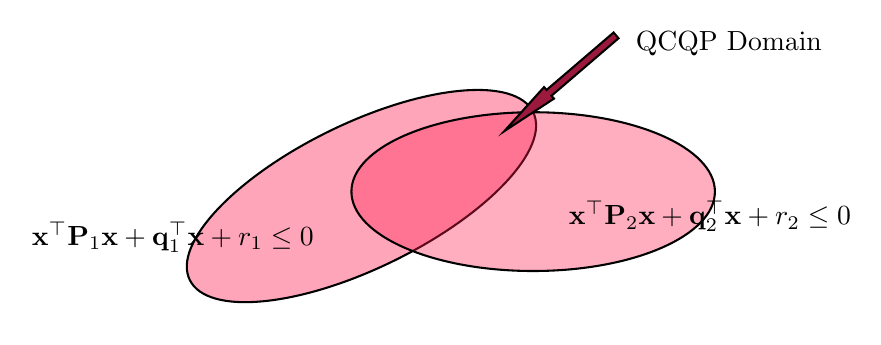
\begin{tikzpicture}[x=0.75pt,y=0.75pt,yscale=-0.75,xscale=0.75]
%uncomment if require: \path (0,300); %set diagram left start at 0, and has height of 300

%Shape: Ellipse [id:dp9898126968799086] 
\draw  [fill=mypink  ,fill opacity=0.4 ] (103.44,199.35) .. controls (92.18,176.27) and (132.43,133.45) .. (193.35,103.71) .. controls (254.27,73.97) and (312.79,68.57) .. (324.06,91.65) .. controls (335.32,114.73) and (295.07,157.55) .. (234.15,187.29) .. controls (173.23,217.03) and (114.71,222.43) .. (103.44,199.35) -- cycle ;
%Shape: Ellipse [id:dp5973223095827915] 
\draw  [fill=mypink  ,fill opacity=0.36 ] (207.31,142.65) .. controls (207.31,114.48) and (259.58,91.65) .. (324.06,91.65) .. controls (388.54,91.65) and (440.81,114.48) .. (440.81,142.65) .. controls (440.81,170.82) and (388.54,193.65) .. (324.06,193.65) .. controls (259.58,193.65) and (207.31,170.82) .. (207.31,142.65) -- cycle ;
%Left Arrow [id:dp11071847750004182] 
\draw  [fill=mydarkpink  ,fill opacity=1 ] (305.5,103.83) -- (331.05,75.5) -- (332.64,77.36) -- (375.73,40.44) -- (378.91,44.15) -- (335.82,81.07) -- (337.41,82.92) -- cycle ;

% Text Node
\draw (0,160) node [anchor=north west][inner sep=0.75pt]    {$\mathbf{x}^\top \mathbf{P}_1 \mathbf{x} + \mathbf{q}_1^\top\mathbf{x} + r_1 \leq 0$};
% Text Node
\draw (345,147) node [anchor=north west][inner sep=0.75pt]    {$\mathbf{x}^\top \mathbf{P}_2 \mathbf{x} + \mathbf{q}_2^\top\mathbf{x} + r_2 \leq 0$};
% Text Node
\draw (388,38) node [anchor=north west][inner sep=0.75pt]   [align=left] {QCQP Domain};


\end{tikzpicture}

\end{center} 
% \caption{AR 601 bipedal robot, Innopolis University}
\end{figure}
 
\end{flushleft}
\end{frame}



\begin{frame}{QCQP to QP and LP}
% \framesubtitle{General form}
\begin{flushleft}

Set $\mathbf{P}_i = \mathbf{0}$ and you get a QP.
%
\begin{equation}
\begin{aligned}
& \underset{\mathbf{x}}{\text{minimize}}
& & \mathbf{x}^\top \mathbf{P}_0 \mathbf{x} + \mathbf{q}_0^\top\mathbf{x}, \\
& \text{subject to}
& & \begin{cases}
    \begin{bmatrix} 
    \mathbf{q}_1^\top \\ ... \\ \mathbf{q}_n^\top
    \end{bmatrix} 
    \mathbf{x} \leq
    \begin{bmatrix} 
    r_1 \\ ... \\ r_n
    \end{bmatrix} \\
    \mathbf{F}\mathbf{x} = \mathbf{g}.
    \end{cases}
\end{aligned}
\end{equation}

Set $\mathbf{P}_0 = \mathbf{0}$ and you get an LP.

\end{flushleft}
\end{frame}




\begin{frame}{Second-order cone programming}
\framesubtitle{General form}
\begin{flushleft}


The general form of a Second-order cone program (SOCP) is:

%
\begin{equation}
\begin{aligned}
& \underset{\mathbf{x}}{\text{minimize}}
& & \mathbf{f}^\top\mathbf{x}, \\
& \text{subject to}
& & \begin{cases}
    ||\mathbf{A}_i\mathbf{x} + \mathbf{b}_i||_2 \leq 
     \mathbf{c}_i^\top \mathbf{x} + d_i, \\
    \mathbf{F}\mathbf{x} = \bo{g}.
    \end{cases}
\end{aligned}
\end{equation}

LP, QP and QCQP are subsets of SOCP.
 
\end{flushleft}
\end{frame}



\begin{frame}{Second-order cone programming}
\framesubtitle{Special cases}
\begin{flushleft}

We can write problem where our domain is a ball as SOCP:
%
\begin{equation}
\begin{aligned}
& \underset{\mathbf{x}}{\text{minimize}}
& & \mathbf{f}^\top\mathbf{x}, \\
& \text{subject to}
& & ||\mathbf{x}||_2 \leq d_i
\end{aligned}
\end{equation}

\bigskip

Same for ellipsoidal constraints:
%
\begin{equation}
\begin{aligned}
& \underset{\mathbf{x}}{\text{minimize}}
& & \mathbf{f}^\top\mathbf{x}, \\
& \text{subject to}
& & ||\mathbf{A}_i\mathbf{x}||_2 \leq d_i
\end{aligned}
\end{equation}
 
\end{flushleft}
\end{frame}




\begin{frame}{SOCP to QCQP}
\framesubtitle{Part 1}
\begin{flushleft}

Set $\mathbf{c}_i = 0$ and $d_i = 0$ and recognize that $||\mathbf{A}_i\mathbf{x} + \mathbf{b}_i||_2 \leq 0$ is the same as $(\mathbf{A}_i\mathbf{x} + \mathbf{b}_i)^\top (\mathbf{A}_i\mathbf{x} + \mathbf{b}_i) \leq 0$

\bigskip
%
\begin{equation}
\begin{aligned}
& \underset{\bo{x}}{\text{minimize}}
& & \bo{f}^\top\bo{x}, \\
& \text{subject to}
& & \begin{cases}
    \bo{x}^\top \bo{A}_i^\top \bo{A}_i \bo{x} + 
    2 \bo{b}_i^\top \bo{A}_i\bo{x} + 
    \bo{b}_i^\top \bo{b}_i  \leq 0\\
    \bo{F}\bo{x} = \bo{g}.
    \end{cases}
\end{aligned}
\end{equation}

\end{flushleft}
\end{frame}




\begin{frame}{SOCP to QCQP}
\framesubtitle{Part 2}
\begin{flushleft}


Now to make the cost quadratic:
%
\begin{equation}
\begin{aligned}
& \underset{\bo{x}}{\text{minimize}}
& & t, \\
& \text{subject to}
& & \begin{cases}
    \bo{x}^\top \bo{A}_0^\top \bo{A}_0 \bo{x} + 
    2 \bo{b}_0^\top \bo{A}_0\bo{x} + 
    \bo{b}_0^\top \bo{b}_0  \leq t\\
    \bo{x}^\top \bo{A}_i^\top \bo{A}_i \bo{x} + 
    2 \bo{b}_i^\top \bo{A}_i\bo{x} + 
    \bo{b}_i^\top \bo{b}_i  \leq 0\\
    \bo{F}\bo{x} = \bo{g}.
    \end{cases}
\end{aligned}
\end{equation}

Which is the same as:
%
\begin{equation}
\begin{aligned}
& \underset{\bo{x}}{\text{minimize}}
& & \mathbf{x}^\top \mathbf{H} \mathbf{x} + \mathbf{f}^\top\mathbf{x}, \\
& \text{subject to}
& & \begin{cases}
    \bo{x}^\top \bo{A}_i^\top \bo{A}_i \bo{x} + 
    2 \bo{b}_i^\top \bo{A}_i\bo{x} + 
    \bo{b}_i^\top \bo{b}_i  \leq 0\\
    \bo{F}\bo{x} = \bo{g}.
    \end{cases}
\end{aligned}
\end{equation}

As long as $\bo{A}_0 = \sqrt{\bo{H}}$, and $\bo{b}_0 = 0.5 \bo{A}_0^{-1} \mathbf{f}$.

\end{flushleft}
\end{frame}




\begin{frame}{Friction cone}
\framesubtitle{Friction and normal reaction force relation}
\begin{flushleft}

\begin{figure}
    \centering
    

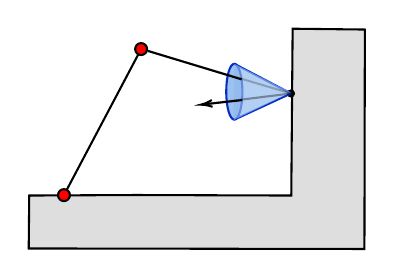
\begin{tikzpicture}[x=0.75pt,y=0.75pt,yscale=-0.5,xscale=0.5]
%uncomment if require: \path (0,300); %set diagram left start at 0, and has height of 300

%Straight Lines [id:da511009501867824] 
\draw    (150.25,190.35) -- (224.6,49.6) ;
%Shape: Polygon [id:ds12621320375323086] 
\draw  [fill={rgb, 255:red, 222; green, 222; blue, 222 }  ,fill opacity=1 ] (440.2,30.8) -- (370.6,30) -- (369.29,190.75) -- (219.79,190.25) -- (116.79,190.75) -- (116.29,241.75) -- (439.79,242.25) -- cycle ;
%Shape: Circle [id:dp8262097043760679] 
\draw  [fill={rgb, 255:red, 0; green, 0; blue, 0 }  ,fill opacity=1 ] (366.13,92.4) .. controls (366.13,90.81) and (367.41,89.53) .. (369,89.53) .. controls (370.59,89.53) and (371.88,90.81) .. (371.88,92.4) .. controls (371.88,93.99) and (370.59,95.28) .. (369,95.28) .. controls (367.41,95.28) and (366.13,93.99) .. (366.13,92.4) -- cycle ;
%Shape: Circle [id:dp2680036705913309] 
\draw  [fill={rgb, 255:red, 255; green, 0; blue, 0 }  ,fill opacity=1 ] (144.5,190.35) .. controls (144.5,187.17) and (147.07,184.6) .. (150.25,184.6) .. controls (153.43,184.6) and (156,187.17) .. (156,190.35) .. controls (156,193.53) and (153.43,196.1) .. (150.25,196.1) .. controls (147.07,196.1) and (144.5,193.53) .. (144.5,190.35) -- cycle ;
%Shape: Ellipse [id:dp3954723668349849] 
\draw  [color={rgb, 255:red, 0; green, 39; blue, 198 }  ,draw opacity=0.97 ][fill={rgb, 255:red, 156; green, 194; blue, 239 }  ,fill opacity=1 ] (306.6,90.7) .. controls (306.6,75.84) and (310.09,63.8) .. (314.4,63.8) .. controls (318.71,63.8) and (322.2,75.84) .. (322.2,90.7) .. controls (322.2,105.56) and (318.71,117.6) .. (314.4,117.6) .. controls (310.09,117.6) and (306.6,105.56) .. (306.6,90.7) -- cycle ;
%Straight Lines [id:da41806140316108764] 
\draw [color={rgb, 255:red, 0; green, 39; blue, 198 }  ,draw opacity=0.97 ][fill={rgb, 255:red, 156; green, 194; blue, 239 }  ,fill opacity=1 ]   (314.4,63.8) -- (369,92.4) ;
%Straight Lines [id:da8734911464392034] 
\draw [color={rgb, 255:red, 0; green, 39; blue, 198 }  ,draw opacity=0.97 ][fill={rgb, 255:red, 156; green, 194; blue, 239 }  ,fill opacity=1 ]   (314.4,117.6) -- (369,92.4) ;

%Flowchart: Merge [id:dp07751328773533905] 
\draw  [color={rgb, 255:red, 0; green, 0; blue, 0 }  ,draw opacity=0 ][fill={rgb, 255:red, 143; green, 185; blue, 237 }  ,fill opacity=0.68 ] (314.4,63.8) -- (313.88,118.01) -- (369.01,91.43) -- cycle ;
%Straight Lines [id:da8106680503102979] 
\draw [color={rgb, 255:red, 0; green, 0; blue, 0 }  ,draw opacity=0.24 ]   (224.6,49.6) -- (369,92.4) ;
%Straight Lines [id:da5735853405821096] 
\draw [color={rgb, 255:red, 0; green, 0; blue, 0 }  ,draw opacity=0.36 ]   (369,92.4) -- (282.2,103.2) ;
%Straight Lines [id:da788051954899972] 
\draw    (321.8,98.8) -- (284.19,102.98) ;
\draw [shift={(282.2,103.2)}, rotate = 353.65999999999997] [color={rgb, 255:red, 0; green, 0; blue, 0 }  ][line width=0.75]    (10.93,-3.29) .. controls (6.95,-1.4) and (3.31,-0.3) .. (0,0) .. controls (3.31,0.3) and (6.95,1.4) .. (10.93,3.29)   ;
%Straight Lines [id:da2615117595464225] 
\draw    (231.29,51.43) -- (321.4,78.8) ;
%Shape: Circle [id:dp33456176340238253] 
\draw  [fill={rgb, 255:red, 255; green, 0; blue, 0 }  ,fill opacity=1 ] (218.85,49.6) .. controls (218.85,46.42) and (221.42,43.85) .. (224.6,43.85) .. controls (227.78,43.85) and (230.35,46.42) .. (230.35,49.6) .. controls (230.35,52.78) and (227.78,55.35) .. (224.6,55.35) .. controls (221.42,55.35) and (218.85,52.78) .. (218.85,49.6) -- cycle ;




\end{tikzpicture}

    % \caption{}
    \label{fig:contact}
\end{figure}

Let $\bo{f}$ be total reaction force, $\bo{f}_n$ be its normal component (perpendicular to the surface locally), also known as normal reaction; and let $\bo{f}_{fr}$ be its tangential component (a vector lying in the tangent plane to the surface, constructed at the contact point), or friction force. Let $\mathbf{e}_n$ be a unit vector, normal to the surface at the point of contact.

\begin{equation}
    \bo{f} =  \bo{f}_n + \bo{f}_{fr}
\end{equation}

\end{flushleft}
\end{frame}



\begin{frame}{Second-order cone programming}
\framesubtitle{Friction cone}
\begin{flushleft}

Defining $\bo{E}_t = [\mathbf{e}_{t, 1}, \ \mathbf{e}_{t, 2}] = \mathcal{L}(\mathbf{e}_n)$ be an orthonormal basis in the tangential space to the surface, we can write:
%
\begin{align*}
\label{friction_cone}
    & \bo{f} = \mathbf{e}_n n + \bo{E}_t \bo{t} & \\
    & \bo{f}_n = \mathbf{e}_n n & \\
    & \bo{f}_{fr} = \bo{E}_t \bo{t} & \\
    & \bo{t} = [t_1, \ t_2]
\end{align*}
%
The friction cone conditions could be written in any of the following ways:
%
\begin{equation}
\label{friction_cone}
    \sqrt{t_1^2 + t_2^2} < \mu n
\end{equation}
%
\begin{equation}
    || \bo{E}_t^\top \mathbf{f} || \leq \mu \mathbf{e}_n^\top \mathbf{f}
\end{equation}
%
where $\mu$ is a friction coefficient.
 
\end{flushleft}
\end{frame}



\begin{frame}{Homework}
% \framesubtitle{Parameter estimation}
\begin{flushleft}

Implement a program that finds right-most point of an intersection of two ellipsoids; visualise the problem and the solution.

\end{flushleft}
\end{frame}




\begin{frame}
	\centerline{Lecture slides are available via Moodle.}
	\bigskip
	\centerline{You can help improve these slides at:}
	\centerline{
		\mygit
	}
	\bigskip
	
	\textcolor{black}{\qrcode[height=1.5in]{https://github.com/SergeiSa/Computational-Intelligence-Slides-Spring-2022}}
	\bigskip
	
	
	\centerline{Check Moodle for additional links, videos, textbook suggestions.}
\end{frame}



\end{document}
